%
% Chapter 1
%
% Unifies results chapters under the framework of human genetics.

\chapter{Introduction}
\label{ch:introduction}

Observable human characteristics or traits are called phenotypes.
Variation in phenotype emerges from the interplay of genetics, environment, and pure chance.
The contributions of each can vary immensely from phenotype to phenotype.
Traits for which genetic variation explains a non-zero percentage of phenotypic variation are heritable.
Virtually all phenotypic traits are heritable to some degree, 
and twin studies provide upper bounds on this heritability by partitioning phenotypic variation into genetic and environmental components \autocite{polderman2015MetaanalysisHeritabilityHuman}.

Genetic variation presents a unique opportunity to probe the causal molecular mechanisms underlying phenotypes.
Information encoded in the genome has phenotypic consequences only after flowing through multiple molecular layers.
% NOTE: There are many mechanisms not explicitly mentioned here: PTMs, epigenetic reg, reverse transcription, RNA editing, but the predominant flow of info holds.
% Also see 
% Koonin, E.V. Does the central dogma still stand?. Biol Direct 7, 27 (2012). https://doi.org/10.1186/1745-6150-7-27
This guiding principle is the central dogma of molecular biology, whereby the flow is directed from DNA to RNA to protein via transcription and translation.
Barring somatic mutation, an individual's genome is fixed at conception, providing a causally upstream anchor that can be measured with relatively little error.
% NOTE: This was why MR was introduced in the context of family-based designs, where parent and child are of the same ancestry \autocite{daveysmith2020MendelLawsMendelian}
A mainstay of the field of human genetics is uncovering the specific genetic variants that contribute to heritability of phenotypes through statistical association of variants and phenotypes.
Although not immune to population-level biases like stratification \autocite{lawson2020PopulationStructureGenetic} and collider bias \autocite{day2016RobustExampleCollider},
genetic association has intrinsic resistance to reverse causality, an issue that permeates observational studies of the causes of human phenotypes.

\section{Genetic association studies for complex traits}

\subsection{Structure and variation of the human genome}

The human genome is over three billion \si{\bp} (base pairs) in length, 
containing \numrange{20000}{25000} protein-coding genes that span \SIrange{1}{3}{\percent} of its length, with the remaining sequence being non-coding \autocite{theencodeprojectconsortium2012IntegratedEncyclopediaDNA,1000genomesprojectconsortium2015GlobalReferenceHuman}.
% Some of the remainder is dedicated to regulatory activities \autocite{theencodeprojectconsortium2012IntegratedEncyclopediaDNA}.
Each diploid cell contains two copies of the genome, organised into 46 chromosomes comprised of 23 maternal-parental pairs: 22 pairs of homologous autosomes and one pair of sex chromosomes.
Variation in the genome between individuals in a population exists in the form of \glspl{SNP}, short indels, and structural variants.
For common population variants with \gls{MAF} \SI{>1}{\percent},
the vast majority (\SI[round-precision=1]{>99.9}{\percent}) are \glspl{SNP} and short indels \autocite{1000genomesprojectconsortium2015GlobalReferenceHuman}.
% https://www.ncbi.nlm.nih.gov/dbvar/content/overview/
% Structural variation (SV) is generally defined as a region of DNA
% approximately 1 kb and larger in size and can include inversions and
% balanced translocations or genomic imbalances (insertions and deletions),
% commonly referred to as copy number variants (CNVs).
On average, a pair of genomes differs by one \gls{SNP} per \SIrange{1000}{2000}{\bp} \autocite{theinternationalsnpmapworkinggroup2001MapHumanGenome}.
Each version of a variant is called an allele; each individual has a maternal and parental allele at each variant.

% The Law of Dominance: An organism with alternate forms of a gene will express the form that is dominant.
% Law of Segregation: states that a diploid organism passes a randomly selected allele for a trait to its offspring, such that the offspring receives one allele from each parent.
% Law of independent assortment: states that genes do not influence each other with regard to the sorting of alleles into gametes; every possible combination of alleles for every gene is equally likely to occur.
The large number of variants in a population are inherited on a smaller number of haplotypes: contiguous stretches of the genome passed through generations via meiotic segregation.
The fundamental sources of genetic diversity, mutation and meiotic recombination, generate new alleles and break apart haplotypes into shorter ones over evolutionary time.
Variants that are physically close on a chromosome are less likely to flank a recombination event, hence are more likely to cosegregate from parent to offspring on the same haplotype (genetic linkage).
Genetic linkage is one source of \gls{LD}: the non-random association of alleles at two variants, differing from expectation based on their population frequencies and the law of independent assortment.
\gls{LD} can be quantified by $r^2$, the squared correlation coefficient between alleles in a specific population \autocite{slatkin2008LinkageDisequilibriumUnderstanding}.
% LD decay takes a really long time, but there are also forces at work that generate or maintain it e.g. drift, selection, admixture, population subdivision, bottlenecks \autocite{slatkin2008LinkageDisequilibriumUnderstanding,visscher2012FiveYearsGWAS}.
%
Recombination events are not distributed uniformly throughout the genome.
The genome is a mosaic of haplotype blocks delimited by recombination hotspots, 
characterised by strong \gls{LD} within blocks, and little \gls{LD} between blocks \autocite{wall2003HaplotypeBlocksLinkage,theinternationalhapmapconsortium2007SecondGenerationHuman} (\cref{fig:intro_haplotypeBlocks}).
The structure of correlated haplotypes reflects a population's unique evolutionary history, and can be used to trace the demography of populations back through time \autocite{karczewski2020AnalyticTranslationalGenetics}.

% NOTE: alternative figure
% Figure S1. Haplotype Block Organization in Human Populations
% https://journals.plos.org/plosgenetics/article?id=10.1371/journal.pgen.0020121
% https://doi.org/10.1371/journal.pgen.0020121.sg001
% (3.6 MB TIF)
\begin{figure}
    \centering
    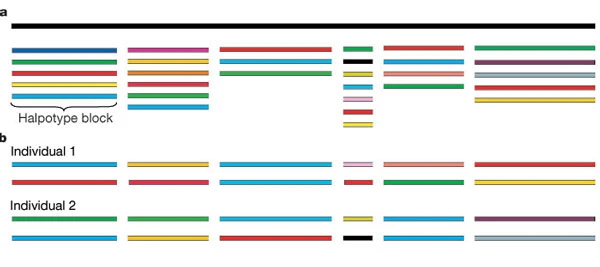
\includegraphics[width=0.8\textwidth,page=1]{mainmatter/figures/chapter_01/paabo2003MosaicThatOur/41586_2003_Article_BFnature01400_Fig3_HTML.png}
    \caption[
        \captionshort{The mosaic structure of human genetic variation.}
    ]{
        \textbf{The mosaic structure of human genetic variation.}
        Large parts of the genome can be divided into haplotype blocks between \SIrange{5}{200}{\kilo\bp} in length, with strong intra-block \gls{LD}.
        For each block, three to seven common haplotypes (indicated by different colors) represent the majority of variation found in humans.
        An individual carries two haplotypes per block, one inherited from each parent.
        The exact structure and diversity of haplotype blocks varies between populations.
        Information on the haplotypes, their locations in the genome, and their frequencies in different populations form a \enquote{haplotype map} of the genome.
        Figure reprinted by permission from Springer Nature: Springer Nature, Nature, \textcite{paabo2003MosaicThatOur}, \textcopyright~2003.
    }
    \label{fig:intro_haplotypeBlocks}
\end{figure}

\subsection{Lessons from the past fifteen years}

Genetic variants can affect heritable traits by impacting the function or regulation of target genes.
How genetic variation contributes to a particular trait defines its genetic architecture: the number of genes affecting the trait; and the frequencies, effect sizes, and interactions of trait-associated alleles \autocite{timpson2018GeneticArchitectureShape,visscher2019Fisher1918Paper}.
The number of genes defines a spectrum of traits from monogenic (where inheritance follows simple Mendelian patterns) to polygenic (where inheritance is complex).
% TODO: add 1 sentence on what complex is.
Proposed architectures differ strikingly among complex traits, 
even for traits with phenotypic similarities like \gls{T1D} and \gls{T2D} \autocite{timpson2018GeneticArchitectureShape}.
Consistently, however, the number of genes and genetic variants affecting a complex trait is large (ranging from dozens to many thousands),
the average effect size of trait-associated variants is small, 
and the contribution of environment is substantial \autocite{hindorff2009PotentialEtiologicFunctional,gibson2011RareCommonVariants,boyle2017ExpandedViewComplex}.

% There are causal variants, but where are they? Two methods that exploit recombination.
% LOD score plots are very similar in concept to GWAS Manhattan plots
Since the 1980s, linkage analysis has been used to map the chromosomal positions and regions (loci) affecting traits by tracing the cosegregation of markers (variants with known positions) with the trait in family pedigrees \autocite{altshuler2008GeneticMappingHuman,ott2011FamilybasedDesignsGenomewide,visscher2012FiveYearsGWAS}.
% \autocite{ott2011FamilybasedDesignsGenomewide}
% Linkage uses a family: since the number of recombinations per generation is small, large chunks of the genome are in linkage in a pedigree. Thus the resolution of linkage is low, but you can cover the genome with just a few hundred markers.
% Also see: https://www.genome.gov/genetics-glossary/LOD-Score for the test statistic for linkage. 
% Association uses population LD: small regions of the genome in very high LD have not been split by recombination over many generations. The resolution is higher, but you need a denser marker set.
Linkage analysis was complemented by early genetic association studies, which largely focused on variants in or near candidate genes selected on the basis of prior biological knowledge \autocite{hirschhorn2002ComprehensiveReviewGenetic}.
These methods saw much success for Mendelian traits, but application to most complex traits proved challenging.
Small average effect sizes meant penetrance was too low to reliably observe cosegregation in pedigrees \autocite{visscher2012FiveYearsGWAS}.
Early candidate gene studies were severely underpowered to detect such small effects \autocite{border2019NoSupportHistorical}.
% TODO: Carl's note: And they also suffered from a poor choice of candidates and inadequate QC.

The past fifteen years have seen the rise of \glspl{GWAS} that systematically test common variants selected in a hypothesis-free manner across the whole genome (\cref{fig:intro_effectSizeVsFrequency}).
Using large sample sizes to overcome small effects and the large multiple testing burden, thousands of associations have been discovered for complex traits and diseases,
many robustly replicated across populations \autocite{visscher2012FiveYearsGWAS,visscher201710YearsGWAS}.
A number of take-home messages have emerged.
%
% Phenotypic variance, usually combines the genotype variance with the environmental variance. Genetic variance has three major components: the additive genetic variance, dominance variance, and epistatic variance.
% NOTE: Polygenic background modifies penetrance of monogenic variants for tier 1 genomic conditions https://www.nature.com/articles/s41467-020-17374-3
Most genetic variance is additive; the contributions of dominance and epistatic interaction are small \autocite{visscher2019Fisher1918Paper}.
Variants with effects on multiple phenotypes (pleiotropy) are widespread \autocite{visscher2012FiveYearsGWAS}.
% It is now appreciated that complex traits have remarkable polygenicity, with many hundreds or thousands of associated loci.
Even traits that are molecular rather than whole-organism phenotypes can be remarkably polygenic, with hundreds to thousands of associated loci \autocite{sinnott-armstrong2020GWASThreeMolecular}.
\Gls{GWAS} sample sizes in the millions are increasingly commonplace,
and the discovery of new associations with ever smaller effects as sample sizes increase shows no sign of plateauing \autocite{tam2019BenefitsLimitationsGenomewide,crouch2020PolygenicInheritanceGWAS}.
% Now the biological interpretation is the greater challenge.
% TODO: add any more big take-homes from: \autocite{gallagher2018PostGWASEraAssociation,tam2019BenefitsLimitationsGenomewide}
% TODO: Carl: This would seem like a good place to bring in the fact that most common variants associated with complex phenotypes are non-coding and are believed to affect disease risk by perturbing the expression of a nearby (and often unknown) gene. You could even add something about how this has hindered our ability to gain biological insights from GWAS and identify drug targets.

% NOTE: see https://www.embopress.org/doi/full/10.15252/emmm.201910316 for a 3D version of this figure.
\begin{figure}
    \centering
    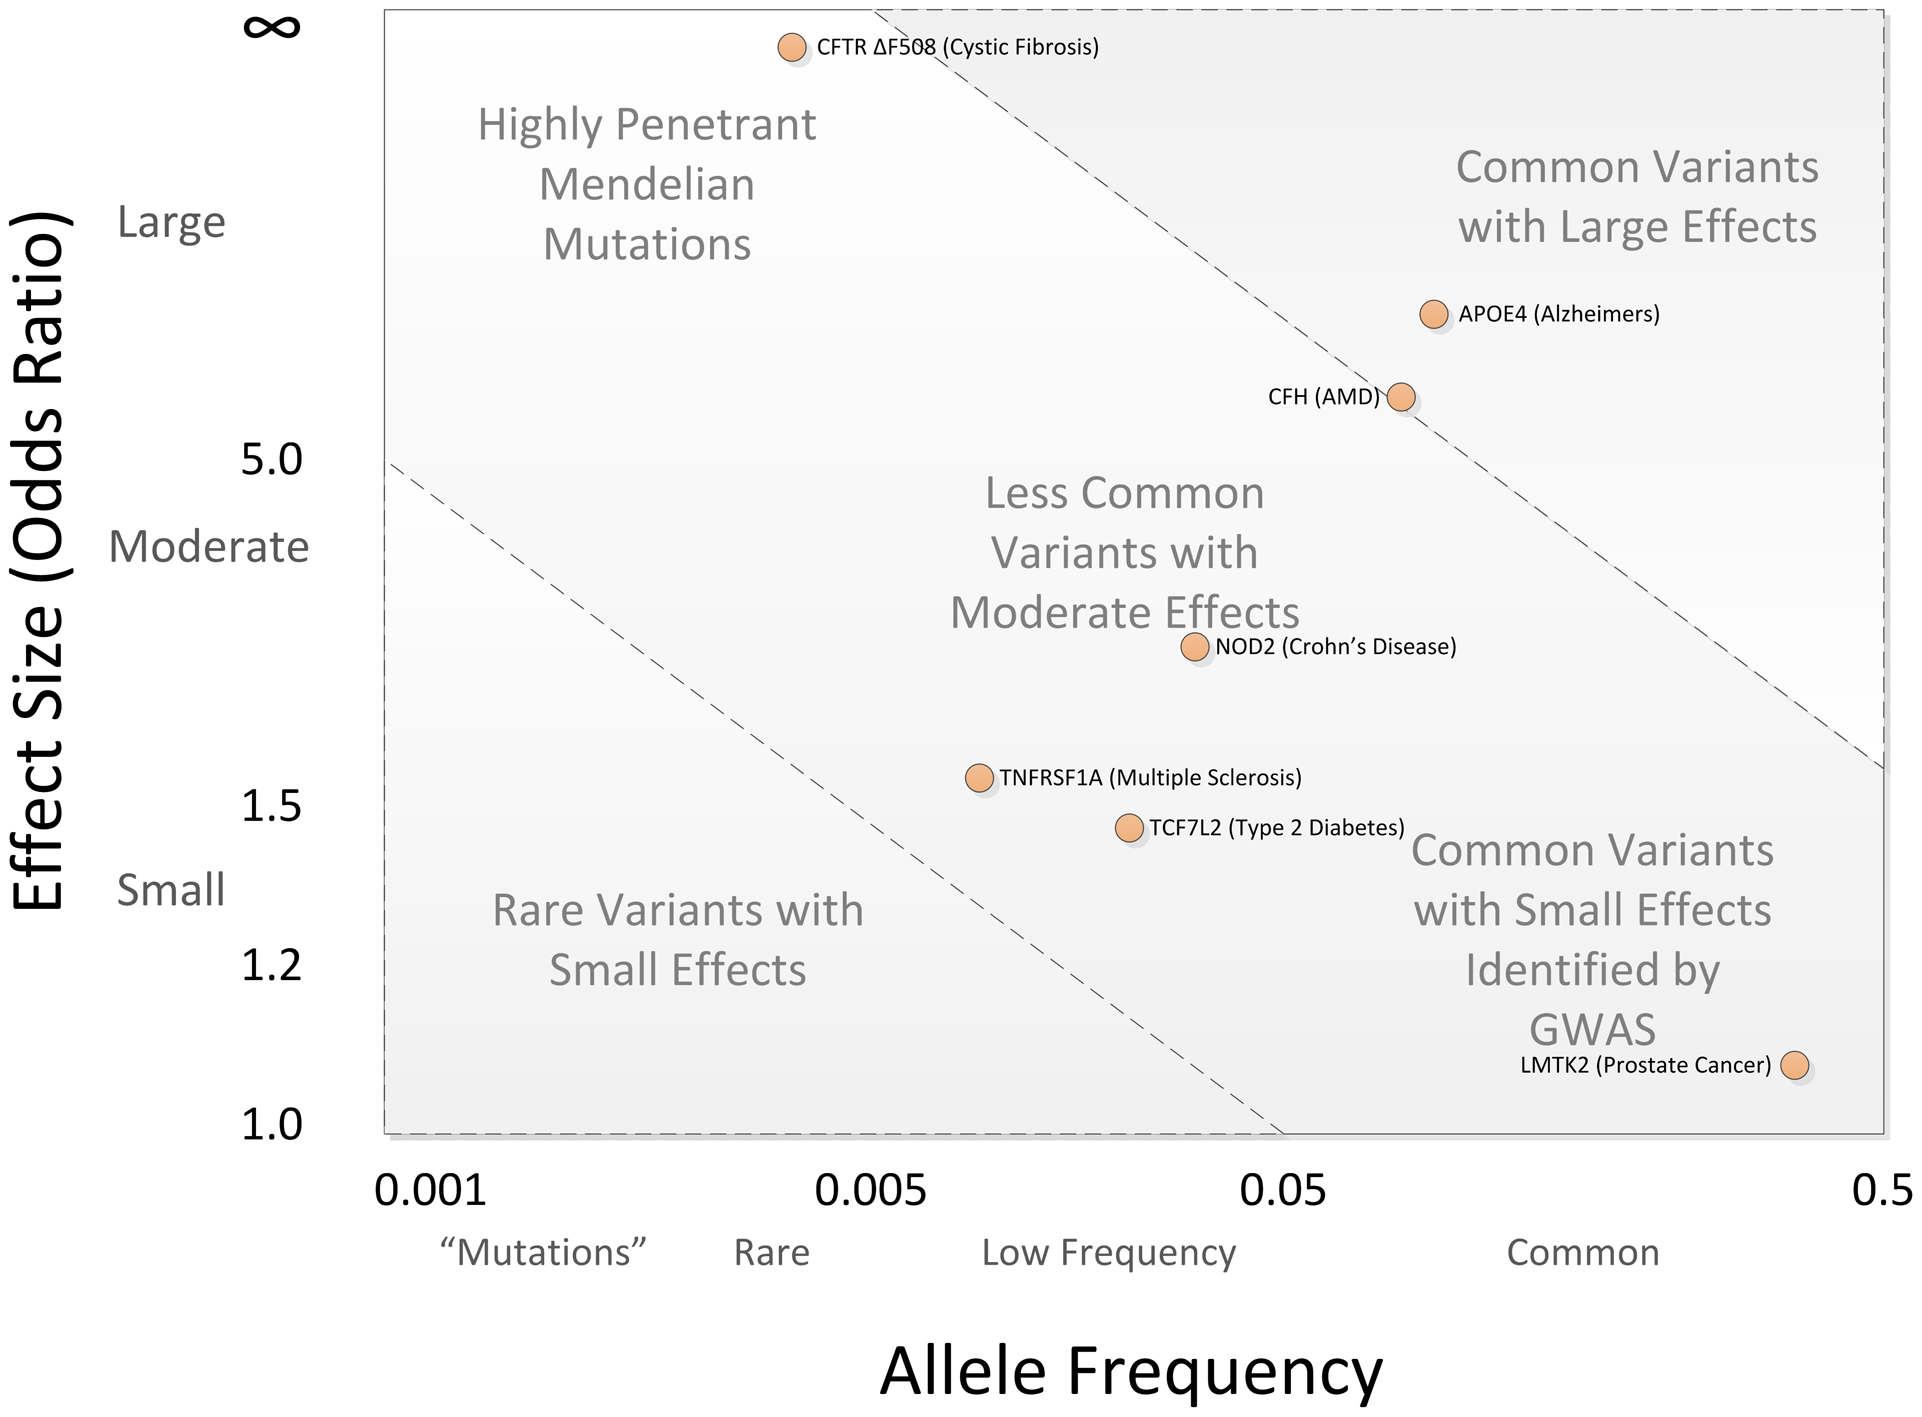
\includegraphics[width=0.9\textwidth,page=1]{mainmatter/figures/chapter_01/bush2012Chapter11GenomeWide/journal.pcbi.1002822.g001.png}
    \caption[
        \captionshort{Effect size and allele frequency of trait-associated genetic variants.}
    ]{
        \textbf{Effect size and allele frequency of trait-associated genetic variants.}
        % Complementary methods are suitable for different trait architectures.
        Different classes of genetic effects require different and complementary methods.
        Linkage analysis is suited to detecting Mendelian variants with large effects.
        \gls{GWAS} is suited to detecting common variants with small effects.
        There are few common variants with large effects due to selection pressure.
        Rare variants with small effects are hard to distinguish from noise without very large samples.
        % TODO: r2 does. D' does not.  % TODO: why?
        They are also poorly tagged by genotyping arrays and difficult to impute.
        Studies focusing on rare variants often employ \gls{WES} or \gls{WGS} to directly type variants.
        Figure reproduced from \textcite{bush2012Chapter11GenomeWide} under the CC BY 4.0 license (\url{creativecommons.org/licenses/by/4.0/legalcode}).
    }
    \label{fig:intro_effectSizeVsFrequency}
\end{figure}

\subsection{From complex trait to locus}

\glspl{GWAS} rely on the tendency of common variants on the same haplotype to be in strong \gls{LD}.
As the number of haplotypes is relatively few, 
it is possible to select a subset of tag variants such that all other known common variants are within a certain \gls{LD} threshold of that subset. 
In practice, there is enough redundancy that the number of variants measured on a modern genotyping array (in the order of \numrange[retain-unity-mantissa=false]{1e5}{1e6}) is sufficient to tag almost all common variants  \autocite{theinternationalhapmapconsortium2005HaplotypeMapHuman,barrett2006EvaluatingCoverageGenomewide}.
Associations with unmeasured variants are indirectly detected through correlation with a tag variant.
Furthermore, as unrelated individuals still share short ancestral haplotypes, 
study samples can be assigned haplotypes from a panel of haplotypes derived from reference samples by matching on directly genotyped variants. 
Genotypes at untyped variants can then be assigned from those haplotypes.
This process---genotype imputation---allows ascertainment of many more variants than are directly genotyped \autocite{das2018GenotypeImputationLarge} and helps to recover rarer variants that are poorly-tagged \autocite{visscher201710YearsGWAS}.
Modern imputation panels enable cost-effective \glspl{GWAS} testing tens of millions of variants as rare as \SIrange[parse-numbers=false]{0.01}{0.1}{\percent} in diverse populations \autocite{taliun2019Sequencing53831}.

Testing large numbers of variants incurs a massive multiple testing burden, 
but acknowledging the correlation between variants due to \gls{LD} and restricting tests to common variants, 
there are only the equivalent of \textapprox{10^6} independent tests in the European genome, 
regardless of the number of tests actually performed \autocite{peer2008EstimationMultipleTesting}.
% TODO: Carl: Providing one sticks to testing common variation. As one lowers the MAF the number of independent tests will increase and the significance threshold should be further decreased.
The field has thus converged on a fixed discovery threshold of $0.05 / 10^6 = \num{5e-8}$ for genome-wide significance in European populations \autocite{jannot2015108HasEmerged}, akin to controlling the \gls{FWER} to below $\alpha = 0.05$ using the Bonferroni correction%
\footnote{
    The Bonferroni correction makes no assumptions about the dependence structure of the \pvalues{}, controlling the \gls{FWER} (probability of at least one type I error) exactly under any structure.
    It is conservative (i.e. controls the \gls{FWER} at a stricter level than the chosen threshold $\alpha$) even for independent tests. 
    In fact, it is always conservative unless the \pvalues{} have strong negative correlations \autocite{goeman2014MultipleHypothesisTesting}.
}.

% \subsection{Missing heritability}
%
% \1 Missing heritability refers to the observation that SNP-based heritability estimates from \gls{GWAS} fall short of additive (narrow-sense) heritability estimates from traditional quantitative methods such as twin studies.
% Perhaps unsurprisingly, it has been hypothesised that the remaining heritability lies in variants that cannot be assessed by \gls{GWAS} due to rarity or small effect.
% A classic example is the heritability of human height, estimated at 80\% by twin studies \autocite{maher2008PersonalGenomesCase},
% where considering only significant associations from \gls{GWAS} explains 5\% \autocite{maher2008PersonalGenomesCase}.
% Consideration of all common variants using mixed models (GCTA) increases the estimate to 45\% \autocite{yang2010CommonSNPsExplain},
% Recent work (GREML-WGS) suggests the full estimate of 80\% might be recoverable by also including rare and poorly tagged variants measured by \gls{WGS} \autocite{wainschtein2019RecoveryTraitHeritability}.
%
% Also see:
% 2007: Wellcome Trust Case Control Consortium landmark GWAS
% 2009: Well-known paper: Finding the missing heritability of complex diseases https://www.ncbi.nlm.nih.gov/pmc/articles/PMC2831613/
% 2018: Revisiting the Missing Heritability of Complex Diseases, Ten Years On https://www.genome.gov/event-calendar/Revisiting-Missing-Heritability-of-Complex-Diseases-Ten-Years-On
%
% NOTE: a second approach to heritability estimation is linkage disequilibrium (LD) score regression.

% \subsection{WGS/WES mitigates the coverage bias of GWAS towards known variation}
%
% \1 approx 10-fold increase in variants per tech upgrade
% \1 WES/WGS is a trade-off between sample size and genomic coverage
%     \2 Allows discovery and association with rare and novel variation, including structural variants.
%     \2 "In addition, other genome-wide scans, such as WES and WGS studies, allow testing for a burden of rare variants across shared functional units (e.g., genes) in a way that is not accessible to GWASs."
% \1 WES (covers about 40Mbp of the genome)
%     \2 covers more of the genome than GWAS
%     \2 but lower n, so lower power to do single variant associations
%     \2 needs 50x: variable coverage due to pulldown
% \1 WGS
%     \2 there is a trade-off between variant capture (n needed to observe variant) and sequencing depth (gives confidence to call variants)
%     \2 20x OK to call 90\% of singletons
%     \2 rare variants, including in nc regions
%         \3 current discovery biases, finding higher effect size vars first
%         \3 burden tests (e.g. SAIGE)
%             \4 review \url{https://www.nature.com/articles/s41576-019-0177-4}
%     \2 also gets structural variants

% \subsection{GWAS isn't designed for rare variation}
%
% There is a limit, the strategy of association is fundamentally unsuited to rare variants.
%
%     Rare Variants Association Analysis in Large-Scale Sequencing Studies at the Single Locus Level
%     https://doi.org/10.1371/journal.pcbi.1004993
%     Despite being extremely successful for common variants in GWA studies [43–46], procedures based on false-positive control are often underpowered in NGS studies involving rare variants (as illustrated in Fig 1).
%     In NGS studies with rare variants, the Signals region often degenerates due to extremely low MAF and high dimensionality.
%
% GWAS arrays also don't tag rare variants very well:
%
% https://www.ncbi.nlm.nih.gov/pmc/articles/PMC3830981/
% When the allele frequencies of two loci are very different, the r2 will never
% be very large. To see this, let's assume pA<<PB and 1-pA≈1. Then the maximum
% r2≈pA/pB*(1-pB), which is <<1 since PA is very small compared to pB. This
% indicates that causal rare variants are mostly likely to be missed in GWAS for
% single marker tests, since GWAS chips are designed to include predominantly
% common variants (e.g. MAF>0.05).
%
% Therefore, GWASs are by design powered to detect association with causal variants that are relatively common in the population.
% \autocite{visscher2012FiveYearsGWAS}

\subsection{From locus to causal variant}

By design, a significant trait-associated variant from a \gls{GWAS} needs not be a variant that causally affects the trait and may only tag a causal variant.
The resolution of the associated locus depends on the local \gls{LD} structure.
% The SNP-SNP correlation matrix
% Fine-mapping is a natural extension of mapping with higher resolution.
Fine-mapping is the process of determining which of the many correlated variants in an associated locus are most likely to be causal,
assuming the causal variants are observed either by direct genotyping or confident imputation.
Due to incomplete power, the causal variants in a locus are not necessarily the ones with the strongest associations \autocite{schaid2018GenomewideAssociationsCandidate}.
Bayesian fine-mapping methods take a variable selection approach, 
assigning each variant a posterior probability of causality.
% TODO: what about multiple?
A credible set of variants likely to contain the causal variant in the locus with some probability can then be determined \autocite{schaid2018GenomewideAssociationsCandidate,wang2020SimpleNewApproach}.
The ability to separate causal and tag variants depends on factors including \gls{LD}, sample size, and the effect size and number of causal variants \autocite{visscher201710YearsGWAS,schaid2018GenomewideAssociationsCandidate}.
% TODO: you could expand this to state how these factors correlate with ability to fine-map.

% \subsection{Polygenic risk scores}
%
% Why care? PRS for prediction.
%
% First PRS
% 13. Wray, N.R., Goddard, M.E., and Visscher, P.M. (2007). Prediction of individual genetic risk to disease from genome-wide association studies. Genome Res. 17, 1520–1528.
%
% Variable prediction accuracy of polygenic scores within an ancestry group
% https://elifesciences.org/articles/48376
%
% Polygenic background modifies penetrance of monogenic variants conferring risk for coronary artery disease, breast cancer, or colorectal cancer
% https://www.medrxiv.org/content/10.1101/19013086v1

\subsection{From causal variant to target gene}

Most causal variants for Mendelian traits are coding variants (nonsense, missense, or frameshift) that impact protein sequence \autocite{chong2015GeneticBasisMendelian}.
In contrast, over \SI{90}{\percent} of \gls{GWAS} loci fall in non-coding regions \autocite{gallagher2018PostGWASEraAssociation},
and often too far from the nearest coding region to be in \gls{LD} \autocite{brodie2016HowFarSNP}.
Even if the causal variants in a locus are fine-mapped, 
one of the greatest challenges following a \gls{GWAS} is prioritising the target genes through which those variants affect the trait.
% TODO: Add statement about the challenges this has posed for biological inference, drug target ID etc. See earlier comment.
% NOTE:
% \autocite{visscher201710YearsGWAS}:
% "For two-thirds of \gls{GWAS}-associated complex trait loci where target genes have been assigned, the implicated gene is not the nearest gene"
% but this is from SMR and TWAS studies, which may have poor performance for assigning causal genes.
%
% NOTE: metabolites: "small molecules, ions, metabolites, vitamins and other biomolecules not directly encoded by genes such as mRNA or proteins"
A reasonable heuristic is to assign the gene with the nearest \gls{TSS} or body as the target, particularly for metabolite traits \autocite{stacey2019ProGeMFrameworkPrioritization}.
For improved accuracy across a variety of complex traits,
integrative methods for gene prioritisation combine variant-to-gene distance with other metrics and data types drawn from numerous external sources \autocite{stacey2019ProGeMFrameworkPrioritization,forgetta2020EffectorIndexPredict,ghoussaini2020OpenTargetsGenetics}.
% TODO provide some details of what these are. You can list eQTLs and the this nicely sets up the next section.

% \subsection{From target gene to candidate drug}
%
% \1 gene to drug
%     \2 Are drug targets with genetic support twice as likely to be approved? Revised estimates of the impact of genetic support for drug mechanisms on the probability of drug approval
%         \3 \url{https://journals.plos.org/plosgenetics/article?id=10.1371/journal.pgen.1008489}
%     GWASing and fine-mapping complex diseases like IBD turns out a large number of common causal variants with small-effect sizes.
%     - Is polygenicity a population or individual property? i.e. are most individual IBD cases driven solely by a distribution of small-effects, or do most patients also have 1 or more large-effect rare variants that point out priority targets for their own personalised treatment?
%     - Do many of these common causal variants e.g. converge to hit on the same pathways?
%     - Otherwise, what is the use of these target discovery pipelines that output ranked lists of target genes? Could a drug designed to modulate a single protein target be expected to work for a large number of patients?
%     \2 how to drug a complex disease with no single 'candidate gene'?
%         \3 e.g. schizo is usually polygenic, future drug development could benefit from taking a multi-target approach \autocite{visscher201710YearsGWAS}
%         \3 e.g. of successful GWAS -> drug target
%             \4 drug targets with genetic support are more likely
%         \3 building allelic series

\section{Gene expression as an intermediate molecular phenotype}

\subsection{Regulation of gene expression}

Gene regulation data are indispensable for gene prioritisation. 
Rather than directly impacting the coding sequence of a gene, 
many non-coding \gls{GWAS} loci are hypothesised to affect traits by affecting the regulation of target gene expression \autocite{gallagher2018PostGWASEraAssociation,cano-gamez2020GWASFunctionUsing}.
Unlike genotype, expression is dynamic across time and space.
Diverse expression programs are responsible for the myriad of cell and tissue types generated during development,
and enable adaptation in response to environmental stimuli.

Expression is the product of eukaryotic transcription, a multi-step process involving interactions between DNA, RNA, and hundreds of proteins \autocite{cramer2019OrganizationRegulationGene}.
% RNA polymerase binds to and moves 3'->5' on the non-coding strand, creating an RNA strand that grows in a 5'->3' direction, with a sequence that corresponds to the coding strand.
Transcription of the pre-\gls{mRNA} is initiated when RNA polymerase and \glspl{TF} form part of a protein complex around the promoter region and \gls{TSS} of a gene.
\Glspl{TF} can also bind to more distant \textit{cis}-regulatory elements such as enhancers and repressors.
These distant regulatory elements interact with the promoter region via DNA looping.
Transcription can only happen in regions of open chromatin, where the packing of DNA-histone complexes (nucleosomes) is loose enough that the DNA is physically accessible to the transcriptional machinery.
Chromatin accessibility is partially determined by histone modifications such as methylation, acetylation, phosphorylation, and ubiquitination \autocite{bannister2011RegulationChromatinHistone}.
% The histone code maps modifications to activation/repression.
The DNA itself can also be modified; methylation at CpG sites in promoters tends to repress transcription \autocite{robertson2000DNAMethylationHealth}.

To form a mature \gls{mRNA}, the pre-\gls{mRNA} is capped at the 5' end by a modified nucleotide and at the 3' end by a poly(A) tail.
% The 3' tail is added after cleaving the pre-mRNA off the rest of the transcribed RNA while the polymerase is still going.
% Splicing is mostly co-transcriptional.
Exons are joined by spliceosomes that cut and rejoin the pre-\gls{mRNA} at one or more pairs of splice sites, excising the intronic sequence between each pair.
% TODO: This sentence needs a polish. Also add a review citation.
The choice of splice sites determines which of many alternatively-spliced transcripts is produced.
% Alternative splicing of pre-mRNA transcripts is regulated by a system of trans-acting proteins (activators and repressors) that bind to cis-acting sites or "elements" (enhancers and silencers) on the pre-mRNA transcript itself. These proteins and their respective binding elements promote or reduce the usage of a particular splice site.
Post-transcriptional regulation of mature \glspl{mRNA} is also possible via RNA editing \autocite{gott2000FunctionsMechanismsRNA} and regulatory elements in the flanking 5' and 3' \glspl{UTR} \autocite{mignone2002UntranslatedRegionsMRNAs}.

% Functional genomics is a field of molecular biology that attempts to describe gene (and protein) functions and interactions.
% Functional genomics focuses on the dynamic aspects such as gene transcription, translation, regulation of gene expression and protein–protein interactions, as opposed to the static aspects of the genomic information such as DNA sequence or structures.
In line with the regulatory hypothesis, \gls{GWAS} variants are heavily enriched in regulatory elements annotated by functional genomics projects (e.g. ENCODE \autocite{theencodeprojectconsortium2012IntegratedEncyclopediaDNA}), including
    % In genetics, DNase I hypersensitive sites (DHSs) are regions of chromatin that are sensitive to cleavage by the DNase I enzyme. In these specific regions of the genome, chromatin has lost its condensed structure, exposing the DNA and making it accessible.
    % DNase-I hypersensitive sites sequencing (DNase-seq; [1–4]) and Assays for Transposase-Accessible Chromatin sequencing (ATAC-seq; [5, 6]) are two widely used protocols for genome-wide identification of open chromatin.
    % The overwhelming majority of disease- and trait-associated variants identified by genome-wide association studies (GWASs) lie in non-coding regions of the genome, and these variants are most strongly enriched in DHSs mapped in disease-relevant cell contexts6,7.
    regions of open chromatin, 
    % ChIP-seq combines chromatin immunoprecipitation (ChIP) with massively parallel DNA sequencing to identify the binding sites of DNA-associated proteins.
    histone binding sites, 
    \gls{TF} binding sites,
    enhancers,
    splice sites,
    and \glspl{UTR}
    \autocite{schaub2012LinkingDiseaseAssociations,maurano2012SystematicLocalizationCommon,farh2015GeneticEpigeneticFine,trynka2015DisentanglingEffectsColocalizing,nasser2020GenomewideMapsEnhancer}.
Furthermore, this enrichment is often observed in particular contexts (tissues, cell types, or cell states \autocite{visscher201710YearsGWAS,gallagher2018PostGWASEraAssociation,cano-gamez2020GWASFunctionUsing}).
% NOTE: cano-gamez2020GWASFunctionUsing contains many examples of genomic feature enrichment methods, including for cell-type and stimulation specific
An example is the enrichment of fine-mapped \glspl{SNP} associated with risk of \gls{IMID} in CD4\textsuperscript{+} T cell enhancers, particularly in enhancers activated after stimulation \autocite{farh2015GeneticEpigeneticFine}.
% NOTE: a good example is T1D vs T2D enrichments, see cano-gamez2020GWASFunctionUsing
These results put forth expression as an important intermediate that links non-coding \gls{GWAS} variants to their associated traits, 
and helps nominate trait-relevant contexts and target genes.
% NOTE: the term endophenotype has a specific definition, so here use intermediate
% Assessing the utility of intermediate phenotypes for genetic mapping of psychiatric disease https://www.ncbi.nlm.nih.gov/pmc/articles/PMC4961231/

% NOTE: pdfbookmarks won't capitalise if \glsfmt variants are used
% \subsection{\Glsfmtfirstpl{eQTL}}
\subsection{Expression quantitative trait loci (eQTLs)}

% \1 The subset of heritable traits that are not only complex but continuous are called quantitative traits, and genetic associations for those traits are called \glspl{QTL}.
Expression is a complex molecular phenotype in itself, with a heritability of \SIrange{15}{30}{\percent} \autocite{gaffney2013GlobalPropertiesFunctional}.
Genome-wide assays for expression, such as microarrays and \gls{RNAseq}, were among the earliest high-throughput technologies developed for quantifying molecular phenotypes.
% TODO: add note on how these technologies work
Genetic loci associated with quantified gene expression are called \glspl{eQTL}.
Large-scale efforts such as the Genotype-Tissue Expression (GTEx) project \autocite{thegtexconsortium2020GTExConsortiumAtlas} have pioneered the study of \glspl{eQTL} and other \glspl{molQTL} over the past decade \autocite{vandiedonck2017GeneticAssociationMolecular}.
% TODO: Can you give more detail about these other molecular QTLs. Above you do discuss the relevant molecular machinery and it would be good to see here some discussion of the big QTL mapping studies for these important traits.
% Recently more focus on other molQTLs e.g. BLUEPRINT for chromatin marks

\gls{eQTL} effect sizes are large relative to variants associated with whole-organism phenotypes,
with the average \gls{eQTL} explaining \SIrange{5}{18}{\percent} of additive genetic variance for its associated gene \autocite{gaffney2013GlobalPropertiesFunctional}.
% NOTE: additive genetic variance is only part of observed variance, but a single variant explaining this much is still large. 
The \glspl{eQTL} with the largest effects tend to be concentrated near the \gls{TSS} of their target gene (\textit{cis}-\glspl{eQTL}), affecting \gls{TF} binding sites and other local regulatory elements.
\glspl{eQTL} further away or on a different chromosome are called \textit{trans}-\glspl{eQTL}.
The exact threshold separating \textit{cis} from \textit{trans} on the same chromosome is arbitrary; \SI{<1}{\mega\bp} and \SI{>5}{\mega\bp} are commonly used thresholds for \textit{cis}- and \textit{trans}-\glspl{eQTL} respectively \autocite{westra2014GenomeFunctionStudying,albert2015RoleRegulatoryVariation,vosa2018UnravelingPolygenicArchitecture}%
\footnote{
    Having a threshold is often a matter of practicality to reduce the number of variants tested.
    Assaying expression is still more costly than array genotyping, so \gls{eQTL} mapping sample sizes are small compared to \glspl{GWAS}.
    Even though \gls{eQTL} effects are relatively large, 
    \gls{eQTL} mapping genome-wide would be equivalent to performing \glspl{GWAS} on thousands of continuous phenotypes,
    incurring enormous computational and multiple testing burdens.
    Studies focused specifically on \textit{trans}-\gls{eQTL} mapping reduce the number of tests in other ways, 
    such as testing only significant \gls{GWAS} variants for \glspl{eQTL} \autocite{vosa2018UnravelingPolygenicArchitecture}.
}.
In general, \gls{eQTL} effect size declines with distance to the \gls{TSS}, and \textit{trans}-\glspl{eQTL} have smaller effects compared to \textit{cis}-\glspl{eQTL} \autocite{vandiedonck2017GeneticAssociationMolecular}.
\textit{Trans}-\glspl{eQTL} often represent \textit{cis}-\glspl{eQTL} of regulatory molecules like \glspl{TF} and RNA-binding proteins that may target many genes in \textit{trans} as master regulators \autocite{fairfax2012GeneticsGeneExpression,albert2015RoleRegulatoryVariation}.
Gathering large enough samples to detect \textit{trans}-\glspl{eQTL} remains a priority,
as most expression heritability is driven by \textit{trans} rather than \textit{cis} effects,
perhaps due to small but wide-reaching effects \autocite{liu2019TransEffectsGene}.
% \2 Currently discovered bulk baseline cis-eQTL have also failed to explain a lot of complex trait heritability.
%     \3 Over many complex traits, a median of 11\% heritability could be explained by mediation of GWAS loci by common (MAF > 0.01) cis-eQTL,
%     and this proportion does not include \textit{trans} or post-transcriptional effects.
%     https://www.nature.com/articles/s41588-020-0625-2
%     Averaging across traits, only 11 ± 2% of heritability was mediated by assayed gene expression levels.

% \subsection{Context-dependent \glsfmtshortpl{eQTL}}
\subsection{Context-dependent eQTLs}
\label{subsec:intro_contextDependenteQTL}

Like expression itself, the effects of \glspl{eQTL} are highly context-dependent \autocite{albert2015RoleRegulatoryVariation,vandiedonck2017GeneticAssociationMolecular}.
When the effect size of an \gls{eQTL} is not the same in all environments, 
but differs depending on the environment, 
the \gls{eQTL} is said to interact with those environments.
This can manifest as a statistical interaction in a regression model with a multiplicative genotype-environment term,
where the effects of environment and genotype on expression are not additive at the chosen scale for measuring expression.
A non-exhaustive list of environmental contexts that have been found to interact with \glspl{eQTL} includes
    sex \autocite{yao2014SexAgeinteractingEQTLs},
    age \autocite{yao2014SexAgeinteractingEQTLs},
    ancestry \autocite{dejager2015ImmVarProjectInsights,nedelec2016GeneticAncestryNatural,quach2017LivingAdaptiveWorld},
    tissue \autocite{nica2011ArchitectureGeneRegulatory,aguet2017GeneticEffectsGene},
    purified cell type \autocite{dimas2009CommonRegulatoryVariation,dejager2015ImmVarProjectInsights,peters2016InsightGenotypePhenotypeAssociations,chen2016GeneticDriversEpigenetic,calderon2019LandscapeStimulationresponsiveChromatin},
    cell type composition in bulk samples \autocite{westra2015CellSpecificEQTL,zhernakova2017IdentificationContextdependentExpression,glastonbury2019CellTypeHeterogeneityAdipose,kim-hellmuth2020CellTypeSpecific},
    cell differentiation stage \autocite{strober2019DynamicGeneticRegulation},
    disease status \autocite{peters2016InsightGenotypePhenotypeAssociations},
    and experimental stimulation (see \cref{subsec:intro_reQTL}).
These contexts can be interdependent;
for example, tissue-dependent effects may arise from a combination of cell type-dependence and varying cell composition between tissues.

A multitude of molecular mechanisms could facilitate genotype-environment interactions at \glspl{eQTL}.
\textcite{fu2012UnravelingRegulatoryMechanisms} mapped \glspl{eQTL} in blood and four non-blood tissues (\cref{fig:intro_reQTLtypes}), 
and proposed mechanisms that might explain discordant effects of an \gls{eQTL} allele on a target gene between tissues,
assuming the \gls{eQTL} disrupts a regulatory factor's binding site.
Different effect sizes of same or opposite signs could arise 
from tissue-dependent effects of the same factor, such as activating expression in one tissue and repressing it in another 
(e.g. due to cofactors, or from binding of different factors in different tissues at the same site).
Effects specific to a tissue could arise from tissue-specific expression of a regulatory factor.
A tissue-specific effect could also reflect tissue-specific target gene expression,
as the \gls{eQTL} effect will be zero in a tissue where the target is not expressed (e.g. due to chromatin inaccessibility).
Tagging of different causal variants in the two tissues, potentially with differing tagging efficiency (i.e. \gls{LD}), could also generate the above scenarios \autocite{fu2012UnravelingRegulatoryMechanisms}.
Furthermore, the complexity of human gene regulation means these mechanisms might be acting at epigenetic, pre-, co-, or post-transcriptional regulatory levels \autocite{gaffney2013GlobalPropertiesFunctional}.
Detection of context-dependent effects merely exposes differences in regulatory architecture between contexts.
Much like in \glspl{GWAS}, going from association to underlying mechanism requires considering data types beyond just genotype and expression.
% TODO: Again, I think you may need to flesh this out more to improve clarity.

\begin{figure}
    \centering
    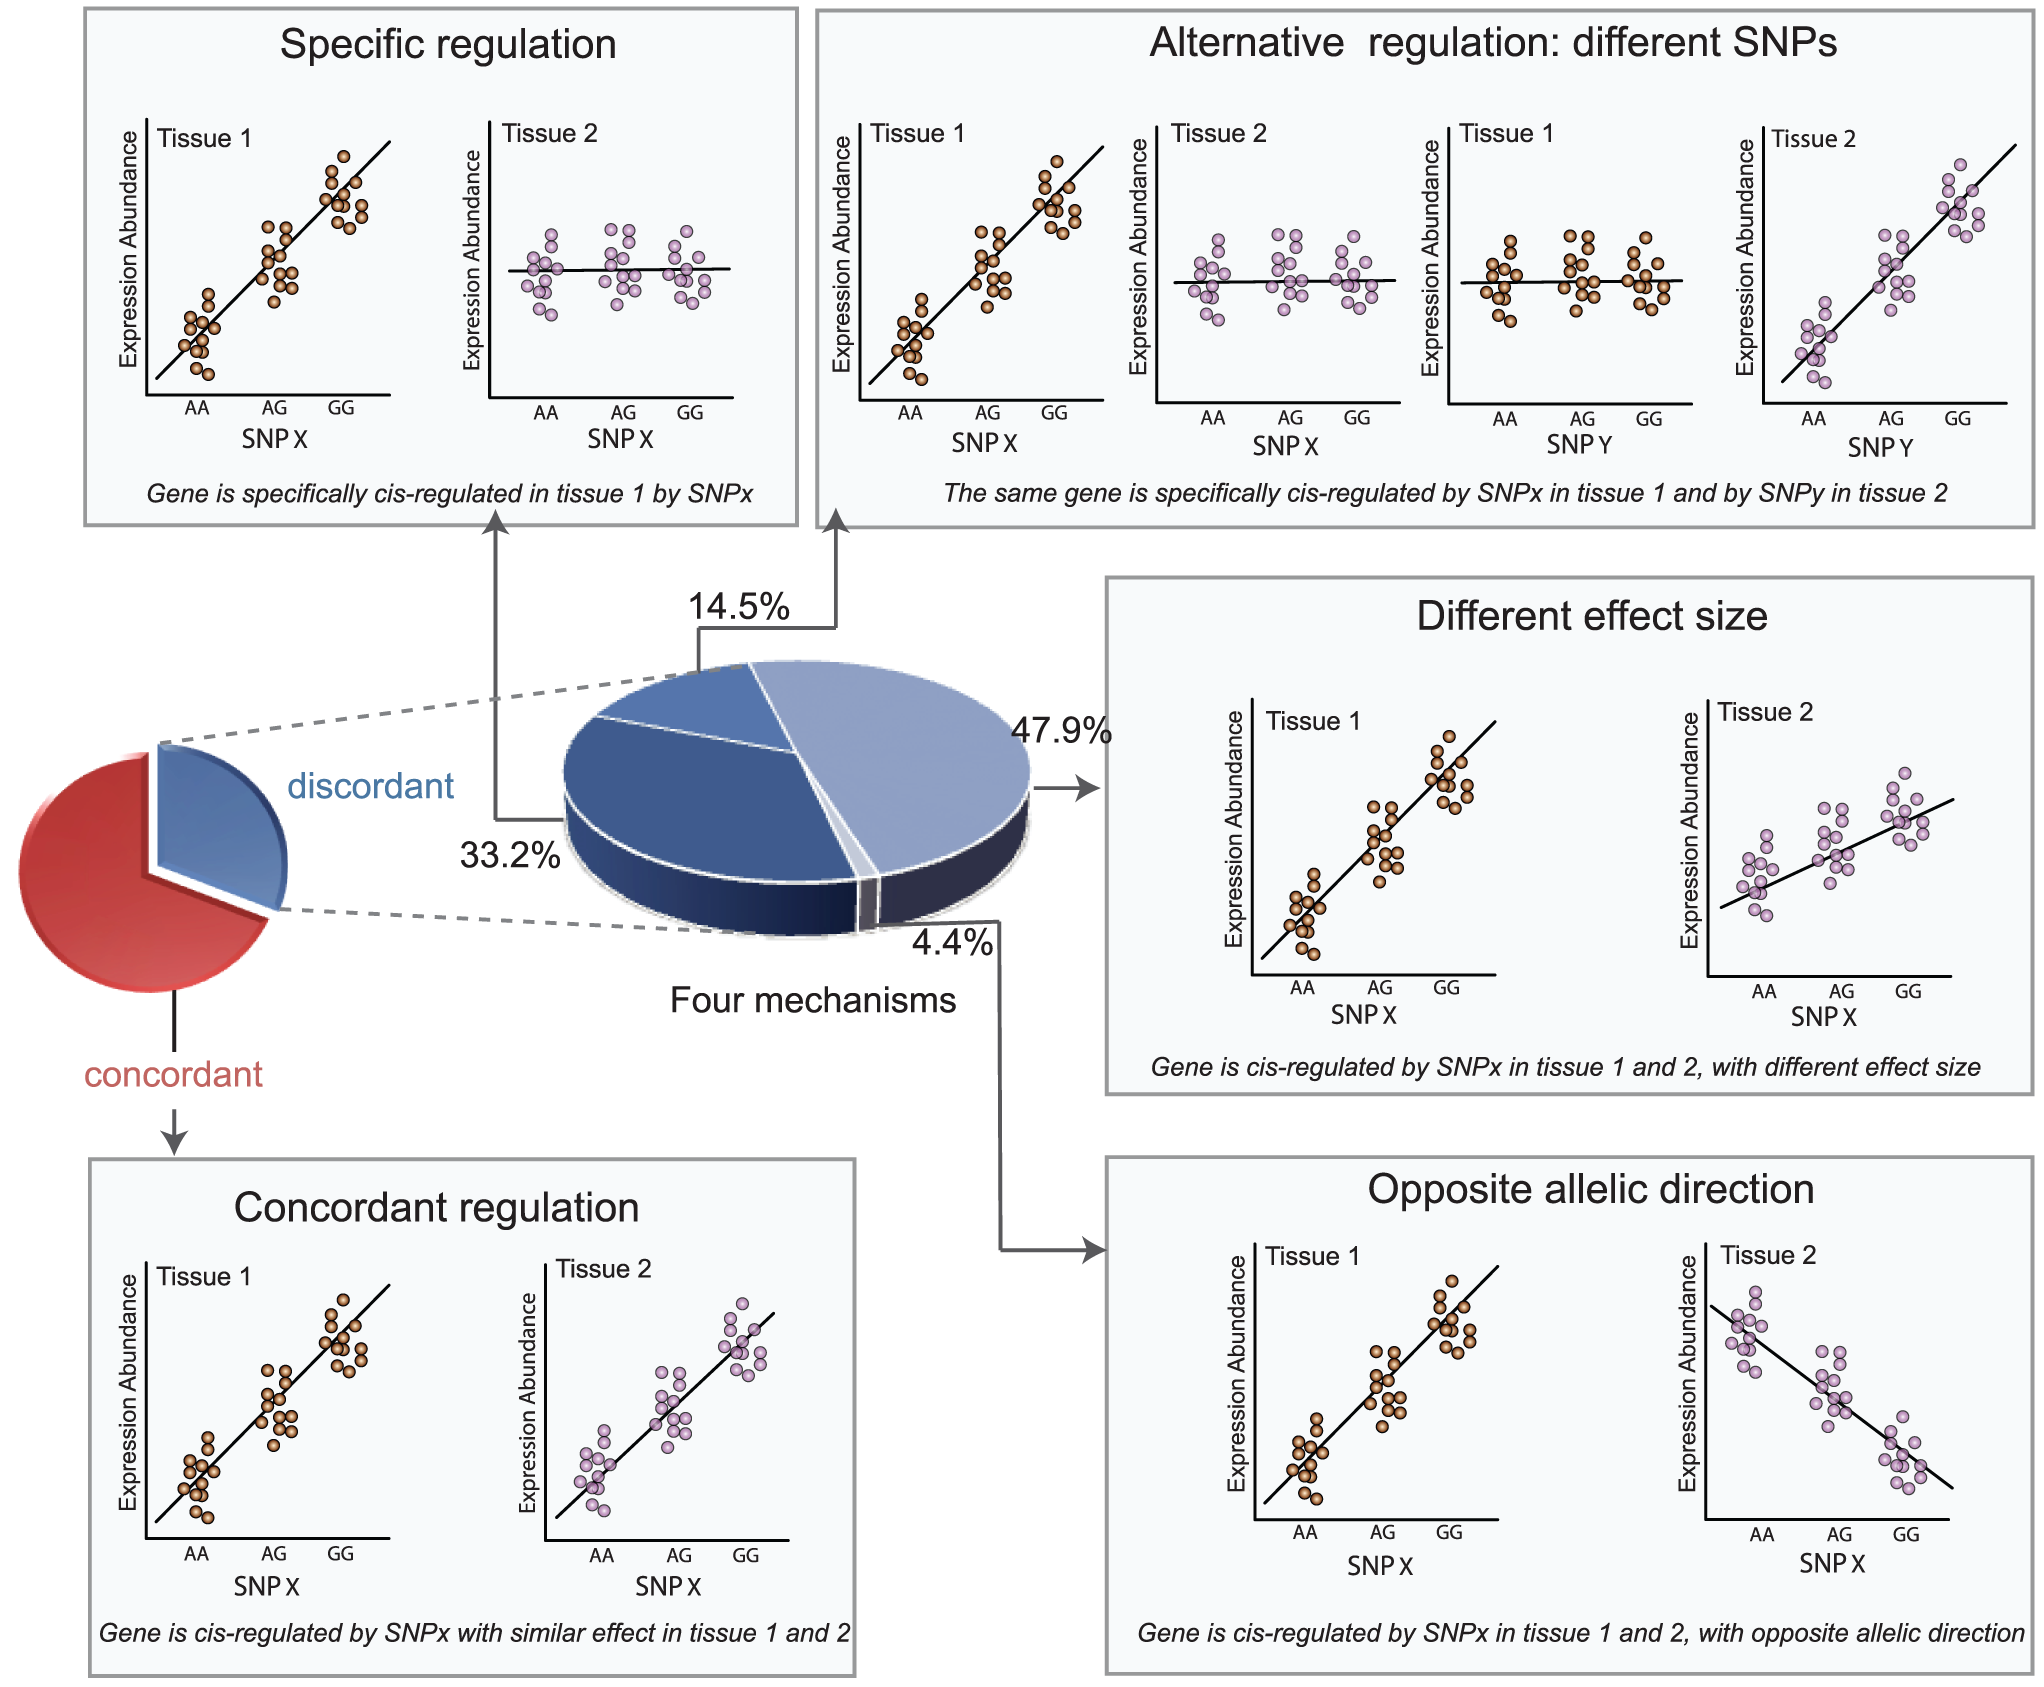
\includegraphics[width=1.0\textwidth,page=1]{mainmatter/figures/chapter_01/fu2012UnravelingRegulatoryMechanisms/journal.pgen.1002431.g002.png}
    \caption[
        \captionshort{Types of tissue-dependent \textit{cis}-\gls{eQTL} effects}.
    ]{
        \textbf{Types of tissue-dependent \textit{cis}-\gls{eQTL} effects}.
        The effect size of an \gls{eQTL} \gls{SNP} on expression can be concordant or discordant between tissues.
        Discordant effects represent genotype-tissue interactions and can be classified into four subtypes.
        Specific regulation refers to a gene with a significant \gls{eQTL} in only one tissue.
        Alternative regulation refers to regulation of the same gene by independent \glspl{SNP} in the two tissues---genes can have multiple \glspl{eQTL} with tissue-specific effects.
        Different effect size refers to an \gls{eQTL} having tissue-dependent effects with concordant sign but discordant magnitude.
        Opposite allelic direction is a tissue-dependent effect where the sign is discordant.
        Pie charts show the proportion of different types of effects in pairwise comparisons of blood and four non-blood tissues by \textcite{fu2012UnravelingRegulatoryMechanisms}.
        Figure reproduced from \textcite{fu2012UnravelingRegulatoryMechanisms} under the CC BY 4.0 license (\url{creativecommons.org/licenses/by/4.0/legalcode}).
    }
    \label{fig:intro_reQTLtypes}
\end{figure}

% \subsection{Immune \glsfmtfullpl{reQTL}}
\subsection{Response eQTLs (reQTLs)}
\label{subsec:intro_reQTL}

A important class of context-dependent \glspl{eQTL} are \glspl{reQTL}, 
where the interacting environment is experimental stimulation,
revealing regulatory effects not detectable in the baseline state \autocite{vandiedonck2017GeneticAssociationMolecular,huang2019GeneticsGeneExpression}.
The vast majority of \gls{reQTL} studies to date have been conducted on immune cells. 
This is not only due to the abundance of immune cells easily accessible in peripheral blood, amenable to purification and stimulation,
but because the immune system is specialised for mounting different responses to different pathogens and perturbations.

When stimulation is applied \textit{in vitro}, variables such as cell type and abundance; and the nature, length, and intensity of stimulation can be precisely controlled.
%
A seminal study by \textcite{barreiro2012DecipheringGeneticArchitecture} mapped \glspl{eQTL} in monocyte-derived \glspl{DC} before and after \SI{18}{\hour} of infection with \textit{Mycobacterium tuberculosis}.
\glspl{reQTL} were detected for 198 genes: 102 specific to the uninfected state and 96 specific to the infected state. 
They observed a 1.4-fold enrichment of \glspl{reQTL} among \gls{GWAS} variants associated with susceptibility to pulmonary tuberculosis,
but no enrichment of \glspl{eQTL} shared between uninfected and infected \glspl{DC}.
From overlap of \glspl{reQTL} and \gls{GWAS} variants,
three genes (\gene{DUSP14}, \gene{ATP6V0A2}, \gene{RIPK2}) were prioritised as candidates affecting tuberculosis susceptibility.
Since then, numerous \textit{in vitro} \gls{reQTL} studies have been conducted with a variety of stimulations (often cytokines, pathogens, or \glspl{PAMP}),
applied to purified \autocite{fairfax2014InnateImmuneActivity,kim2014CharacterizingGeneticBasis,hu2014RegulationGeneExpression,lee2014CommonGeneticVariants,caliskan2015HostGeneticVariation,quach2016GeneticAdaptationNeandertal,kim-hellmuth2017GeneticRegulatoryEffects,alasoo2018SharedGeneticEffects,gate2018GeneticDeterminantsCoaccessible,schmiedel2018ImpactGeneticPolymorphisms,alasoo2019GeneticEffectsPromoter,calderon2019LandscapeStimulationresponsiveChromatin,devries2020IntegratingGWASBulk,huang2020NeonatalGeneticsGene}
or mixed cell types \autocite{caliskan2015HostGeneticVariation,manry2017DecipheringGeneticControl}.

A complementary approach is \gls{reQTL} mapping with \textit{in vivo} stimulation.
An isolated mixture of cells \textit{in vitro} cannot hope to replicate the innumerable interactions involved in human immune response.
\textit{In vivo} designs suit whole-organism stimulations and response phenotypes,
such as vaccination and vaccine-induced antibody response.
%
Published \textit{in vivo} \gls{reQTL} studies are comparatively few.
\textcite{idaghdour2012EvidenceAdditiveInteraction} mapped whole blood \glspl{eQTL} in 94 West African children admitted to hospital for malaria and 61 age-matched controls.
\glspl{reQTL} with a significant case-genotype interaction were detected for five genes:
\gene{PRUNE2}, \gene{SLC39A8}, \gene{C3AR1}, \gene{PADI3}, and \gene{UNC119B}.
As \gene{SLC39A8} is upregulated with T cell activation, a postulation was made that T cell activation is important to malaria infection response.
In \textcite{franco2013IntegrativeGenomicAnalysis}, whole blood \glspl{eQTL} were mapped in 247 healthy adults given \gls{TIV}.
Twenty genes involved in membrane trafficking and antigen processing were prioritised to be important to vaccine response,
on account of having post-vaccination \glspl{reQTL} or differential expression, and an expression correlation with antibody response.
\textcite{lareau2016InteractionQuantitativeTrait} focused on epistatic effects of \gls{SNP}-\gls{SNP} interactions on expression fold-change after smallpox vaccination in 183 individuals.
Eleven significant interactions were found where the effect of two independent \glspl{SNP} on expression was non-additive.
Apoptosis-related genes (e.g. \gene{TRAPPC4}, \gene{ITK}) were enriched among target genes.
Most recently, \textcite{davenport2018DiscoveringVivoCytokineeQTL}
mapped whole blood \glspl{eQTL} in 157 \gls{SLE} patients in a phase II clinical trial of an anti-IL-6 monoclonal antibody.
Nine \glspl{reQTL} with effect sizes magnified by drug exposure were found to disrupt the binding site of IRF4,
highlighting it as a key regulatory factor downstream of IL-6.
%
Overall, \textit{in vivo} \gls{reQTL} studies have delivered insight into the biology of a diverse set of whole-organism phenotypes.
However, ethical requirements can limit sample size and choice of stimulation.
Many environmental factors (e.g. diet, lifestyle, immune exposures) cannot be controlled, 
potentially leading to greater experimental noise compared to \textit{in vitro} designs, and complicating interpretation of results.
% TODO: This section could certainly be fleshed out more.

% \subsection{Gene prioritisation using \glsfmtshortpl{eQTL}}
\subsection{Gene prioritisation using eQTLs}
\label{subsec:intro_genePrioritisationUsingeQTL}

\glspl{eQTL} are enormously valuable for target gene prioritisation after \gls{GWAS}.
They propose both target gene and mechanism of action, where the effect of variant on complex trait is mediated through expression.
\Gls{GWAS} variants for many traits are indeed enriched for \glspl{eQTL} \autocite{nicolae2010TraitAssociatedSNPsAre}, 
but care must be taken when conducting enrichment analyses to avoid false positives due to the abundance of \glspl{eQTL}.
At current sample sizes, \SIrange{60}{80}{\percent} of genes have at least one detectable \gls{eQTL} \autocite{vandiedonck2017GeneticAssociationMolecular,vosa2018UnravelingPolygenicArchitecture}.
% NOTE: nominal threshold
% and half of common variants are \textit{cis}-\glspl{eQTL} for at least one gene \autocite{liu2019AbundantAssociationsGene}.
Assuming that a locus is associated with both a trait of interest and with expression of a particular gene,
how can one separate the scenario where the same causal variants affect both trait and expression (pleiotropy) from coincidental overlap between distinct sets of causal variants that may possibly be in \gls{LD}?
Bayesian colocalisation methods address this problem by extending Bayesian fine-mapping methods to multiple phenotypes \autocite{burgess2018InferringCausalRelationships,wallace2020ElicitingPriorsRelaxing,hukku2020ProbabilisticColocalizationGenetic}.
% They don't really extend fine-mapping because they don't try to define a causal variant.
Using information from all measured variants in the locus, 
they estimate the posterior probability that the same causal variants are associated with both phenotypes,
distinguishing pleiotropy from \gls{LD}.

Given the effect of an \gls{eQTL} can be starkly context-dependent, 
\gls{eQTL} datasets from trait-relevant contexts are most useful for gene prioritisation.
For instance, immune \textit{in vitro} \glspl{reQTL} are enriched more so than non-\glspl{reQTL} among \gls{GWAS} associations for immune-related phenotypes, 
such as susceptibility to infectious \autocite{barreiro2012DecipheringGeneticArchitecture,manry2017DecipheringGeneticControl} and immune-mediated diseases \autocite{manry2017DecipheringGeneticControl,kim-hellmuth2017GeneticRegulatoryEffects}.
% Also see: https://genome.cshlp.org/content/26/12/1627
% High-throughput allele-specific expression across 250 environmental conditions
% Recently, allele-specific expression (ASE) analysis emerged as a powerful tool to identify GxE interactions in gene expression patterns by exploiting naturally occurring environmental exposures. Here we characterized genetic effects on the transcriptional response to 50 treatments in five cell types. We discovered 1455 genes with ASE (FDR < 10%) and 215 genes with GxE interactions. We demonstrated a major role for GxE interactions in complex traits. Genes with a transcriptional response to environmental perturbations showed sevenfold higher odds of being found in GWAS.0
Supplementing shared \gls{eQTL} effects with cell type-specific \gls{eQTL} effects finds many additional colocalisations with complex traits \autocite{kundu2020GeneticAssociationsRegulatory,kim-hellmuth2020CellTypeSpecific}.
The increasing number of context-dependent \gls{eQTL} datasets available for large-scale colocalisation analyses means \glspl{eQTL} can propose not just target gene and mechanism, but also the specific environments most relevant to a trait.

% NOTE:
% coloc also helps finemap
% coloc can also can help fine mapping, as large effect = smaller n required = able to do denser genotype by e.g. wgs, so smaller credible sets at much lower sample sizes
% "Overall, our findings suggest that fine-mapping applied to disease-colocalising regulatory QTLs can enhance the discovery of putative causal disease variants and provide insights into the underlying causal genes and molecular mechanisms."
% https://www.biorxiv.org/content/10.1101/2020.01.15.907436v1

\section{Phenotypes of immune response}

\subsection{An overview of the immune system}

Immunology began as the study of host defense against infection \autocite{murphy2016ChapterBasicConcepts}.
It is now recognised that the immune system is also involved in pathogenesis of diverse conditions encompassing allergic diseases, autoimmune and immune-mediated diseases, and cancer.
% NOTE: autoimmune disease e.g. coeliac disease, where the trigger is loss of tolerance against gluten, and autoantibodies form against the body's own enzymes
This subsection provides a basic overview of parts of the immune system relevant to this thesis.

% <two arms>
The two major arms of the immune response are the innate and adaptive response.
The innate response is rapid and non-specific, 
occurring in the first few minutes to days after the initial (primary) exposure to infection.
This triggers the adaptive response, which takes days to weeks to develop, 
but delivers a powerful and specific response capable of eliminating pathogens that have evaded the innate response.
The adaptive response can also create immunological memory lasting years to decades,
where re-exposure to the same pathogen induces a faster and more powerful recall response%
\footnote{
    There is increasing evidence the innate immune system also has a form of immunological memory \autocite{dominguez-andres2020SpecificsInnateImmune}.
}.
Both arms distinguish self from non-self through complex interactions between many cell types via surface receptors and signalling molecules.

% <two lineages>
Immune cell types differentiate from common myeloid progenitor or common lymphoid progenitors,
which themselves are descended from pluripotent \glspl{HSC} in the bone marrow.
By and large, the cells of the innate response are of the myeloid lineage, 
and the cells of the adaptive response are of the lymphoid lineage.
Immune cells are also called leukocytes or white-blood cells as many types can be found in peripheral blood, 
but certain types are confined to tissues or parts of the lymphatic system.

% <innate cell types>
% Macrophages, neutrophils, and dendritic cells are sensor cells
Innate response begins with the detection of pathogens by phagocytotic sensor cells---primarily neutrophils, tissue-resident macrophages, and \glspl{DC}.
These cells express \glspl{PRR} that recognise conserved \glspl{PAMP} not present in host cells,
% "Some PRRs are transmembrane proteins, such as the Toll-like receptors (TLRs) that detect PAMPs derived from extracellular bacteria or bacteria taken into vesicular pathways by phagocytosis.
% Other PRRs are cytoplasmic proteins, such as the NOD-like receptors (NLRs) that sense intracellular bacterial invasion."
then secrete small proteins (cytokines) that trigger the inflammatory response:
a massive recruitment of multiple cell types from blood into infected tissues.
Recruitment is partially mediated by a family of cytokines called chemokines, which chemically attract immune cells by creating a concentration gradient (chemotaxis). 
% Inflammation is usually neutrophils recruited first, then monocytes.
Recruited neutrophils clear pathogens by phagocytosis and secrete antimicrobial molecules by degranulation.
\Gls{NK} cells detect and kill virus-infected and tumour cells.
Circulating monocytes migrate to the site of infection and differentiate into macrophages and \glspl{DC}.
% TODO: CD14+CD16++ non-classical monocytes, classical CD14++CD16-, intermediate CD14++CD16+ subsets
Macrophages perform phagocytosis, modulate inflammation, and can also engage in antigen-presentation---but it is \glspl{DC} that are considered to be the specialist \gls{APC} type.
% TODO: macrophage subsets
% TODO: DC myeloid and lymphoid
% Antigen-presenting cells fall into two categories: professional and non-professional.
% Those that express MHC class II molecules along with co-stimulatory molecules and pattern recognition receptors are often called professional antigen-presenting cells.[1]
% The non-professional APCs express MHC class I molecules, just like most human cells.
Antigen-presentation by \glspl{DC} is a key link between the innate and adaptive responses.
% "The primary lymphoid organs are the bone marrow and the thymus, an organ in the upper chest.
% The peripheral lymphoid organs comprise the lymph nodes, the spleen, and the mucosal lymphoid tissues of the gut, the nasal and respiratory tract, the urogenital tract, and other mucosa."
% Antigen-presentation happens in peripheral lymphoid organs.

% Lymphocytes include natural killer cells (which function in cell-mediated, cytotoxic innate immunity),
% T cells (for cell-mediated, cytotoxic adaptive immunity),
% and B cells (for humoral, antibody-driven adaptive immunity).[2][3]
% They are the main type of cell found in lymph, which prompted the name "lymphocyte".[4]
The main forces of the adaptive response comprise B and T lymphocytes.
% B and T cells are sources from bone marrow common lymphoid progenitors.
% B and T cells complete their development to naive lymphocytes in the bone marrow and thymus respectively.
% \todo{maintain a pool naive lymphocytes, each having a receptor specific for a different possible antigen}
Naive lymphocytes express antigen receptors that recognise parts of specific antigens called epitopes.
When they encounter this antigen, they activate, proliferate (clonal expansion), then differentiate into effector cells.
To initiate adaptive response,
% CD8 and CD4 function in antigen recognition by recognizing different regions of MHC molecules and by being involved in the signaling of the T-cell receptor that is engaged with its antigen. Thus, CD4 and CD8 are known as co-receptors and they provide a functional difference between CD8 and CD4 T cells,
% Because CD8 recognizes a region of the MHC class I protein while CD4 recognizes a region of MHC class II protein, the two co-receptors functionally distinguish T cells. Therefore, CD8 T cells selectively recognize peptides that are bound to MHC class I molecules, while CD4 T cells recognize peptides presented by MHC class II.
% MHC polymorphism affects antigen recognition by T cells by influencing both peptide binding and the contacts between T-cell receptor and MHC molecule.
% \todo{add TCR}
CD4\textsuperscript{+} (helper) T cells recognise peptide fragments from the antigen presented in a complex with \gls{MHC} class II on the surface of \glspl{APC}.
% TODO th1, th2 main subsets, th17, treg
% Binding requires TCR (CD3), CD4, MHC class II and costimulatory factors.
CD4\textsuperscript{+} T cells then differentiate into several subsets; these activate and regulate other immune cell types such as macrophages, CD8\textsuperscript{+} T cells and B cells.
Activated CD8\textsuperscript{+} (cytotoxic) T cells recognise antigens presented by \gls{MHC} class I on infected cells and directly kill the cell.
% \todo{distinguish plasmablast/plasma cell and add long lived plasma cells}
% \todo{add B cell activation mechanism by CD4, BCR}
Activated B cells differentiate into plasma cells that secrete large quantities of antibodies, the soluble form of the \gls{BCR}.
% TODO:
% These bind specifically to the same that which identify and neutralise pathogens by specific binding to an epitope on the target antigen.
Antibody-mediated immunity is also called humoral immunity,
whereas T cell and innate immune responses comprise cell-mediated immunity.
A small subset of activated B and T cells can become memory cells, responsible for long-term immunological memory.
% TODO: add where these reside, and how they reencounter antigens

\subsection{High-throughput immunology}

% TODO: read pulendran2020ScienceMedicineHuman
To understand the immune system and its intricate interactions,
\enquote{systems immunology} studies take a holistic rather than reductionist experimental approach \autocite{davis2017SystemsImmunologyJust,villani2018SystemsImmunologyLearning,pulendran2020ScienceMedicineHuman}.
The basic principle is the same: experimentally perturb the immune system and observe its response.
Drugs and vaccines can be used as safe and synchronised perturbations---one of the largest subfields of systems immunology is systems vaccinology, which I review in \cref{subsec:hird_dge_intro_systemsVaccFlu}.
A range of high-throughput technologies are applied to measure response at many layers of the immune system (\cref{fig:intro_sysImmunology}).
Longitudinal designs are common, aiming to sample timepoints corresponding to baseline, innate, and adaptive immunity.
The complexity of the immune response presents a major challenge,
with the richness of sampling required often restricting the sample sizes of systems immunology studies due to cost and logistics.

\begin{figure}
    \centering
    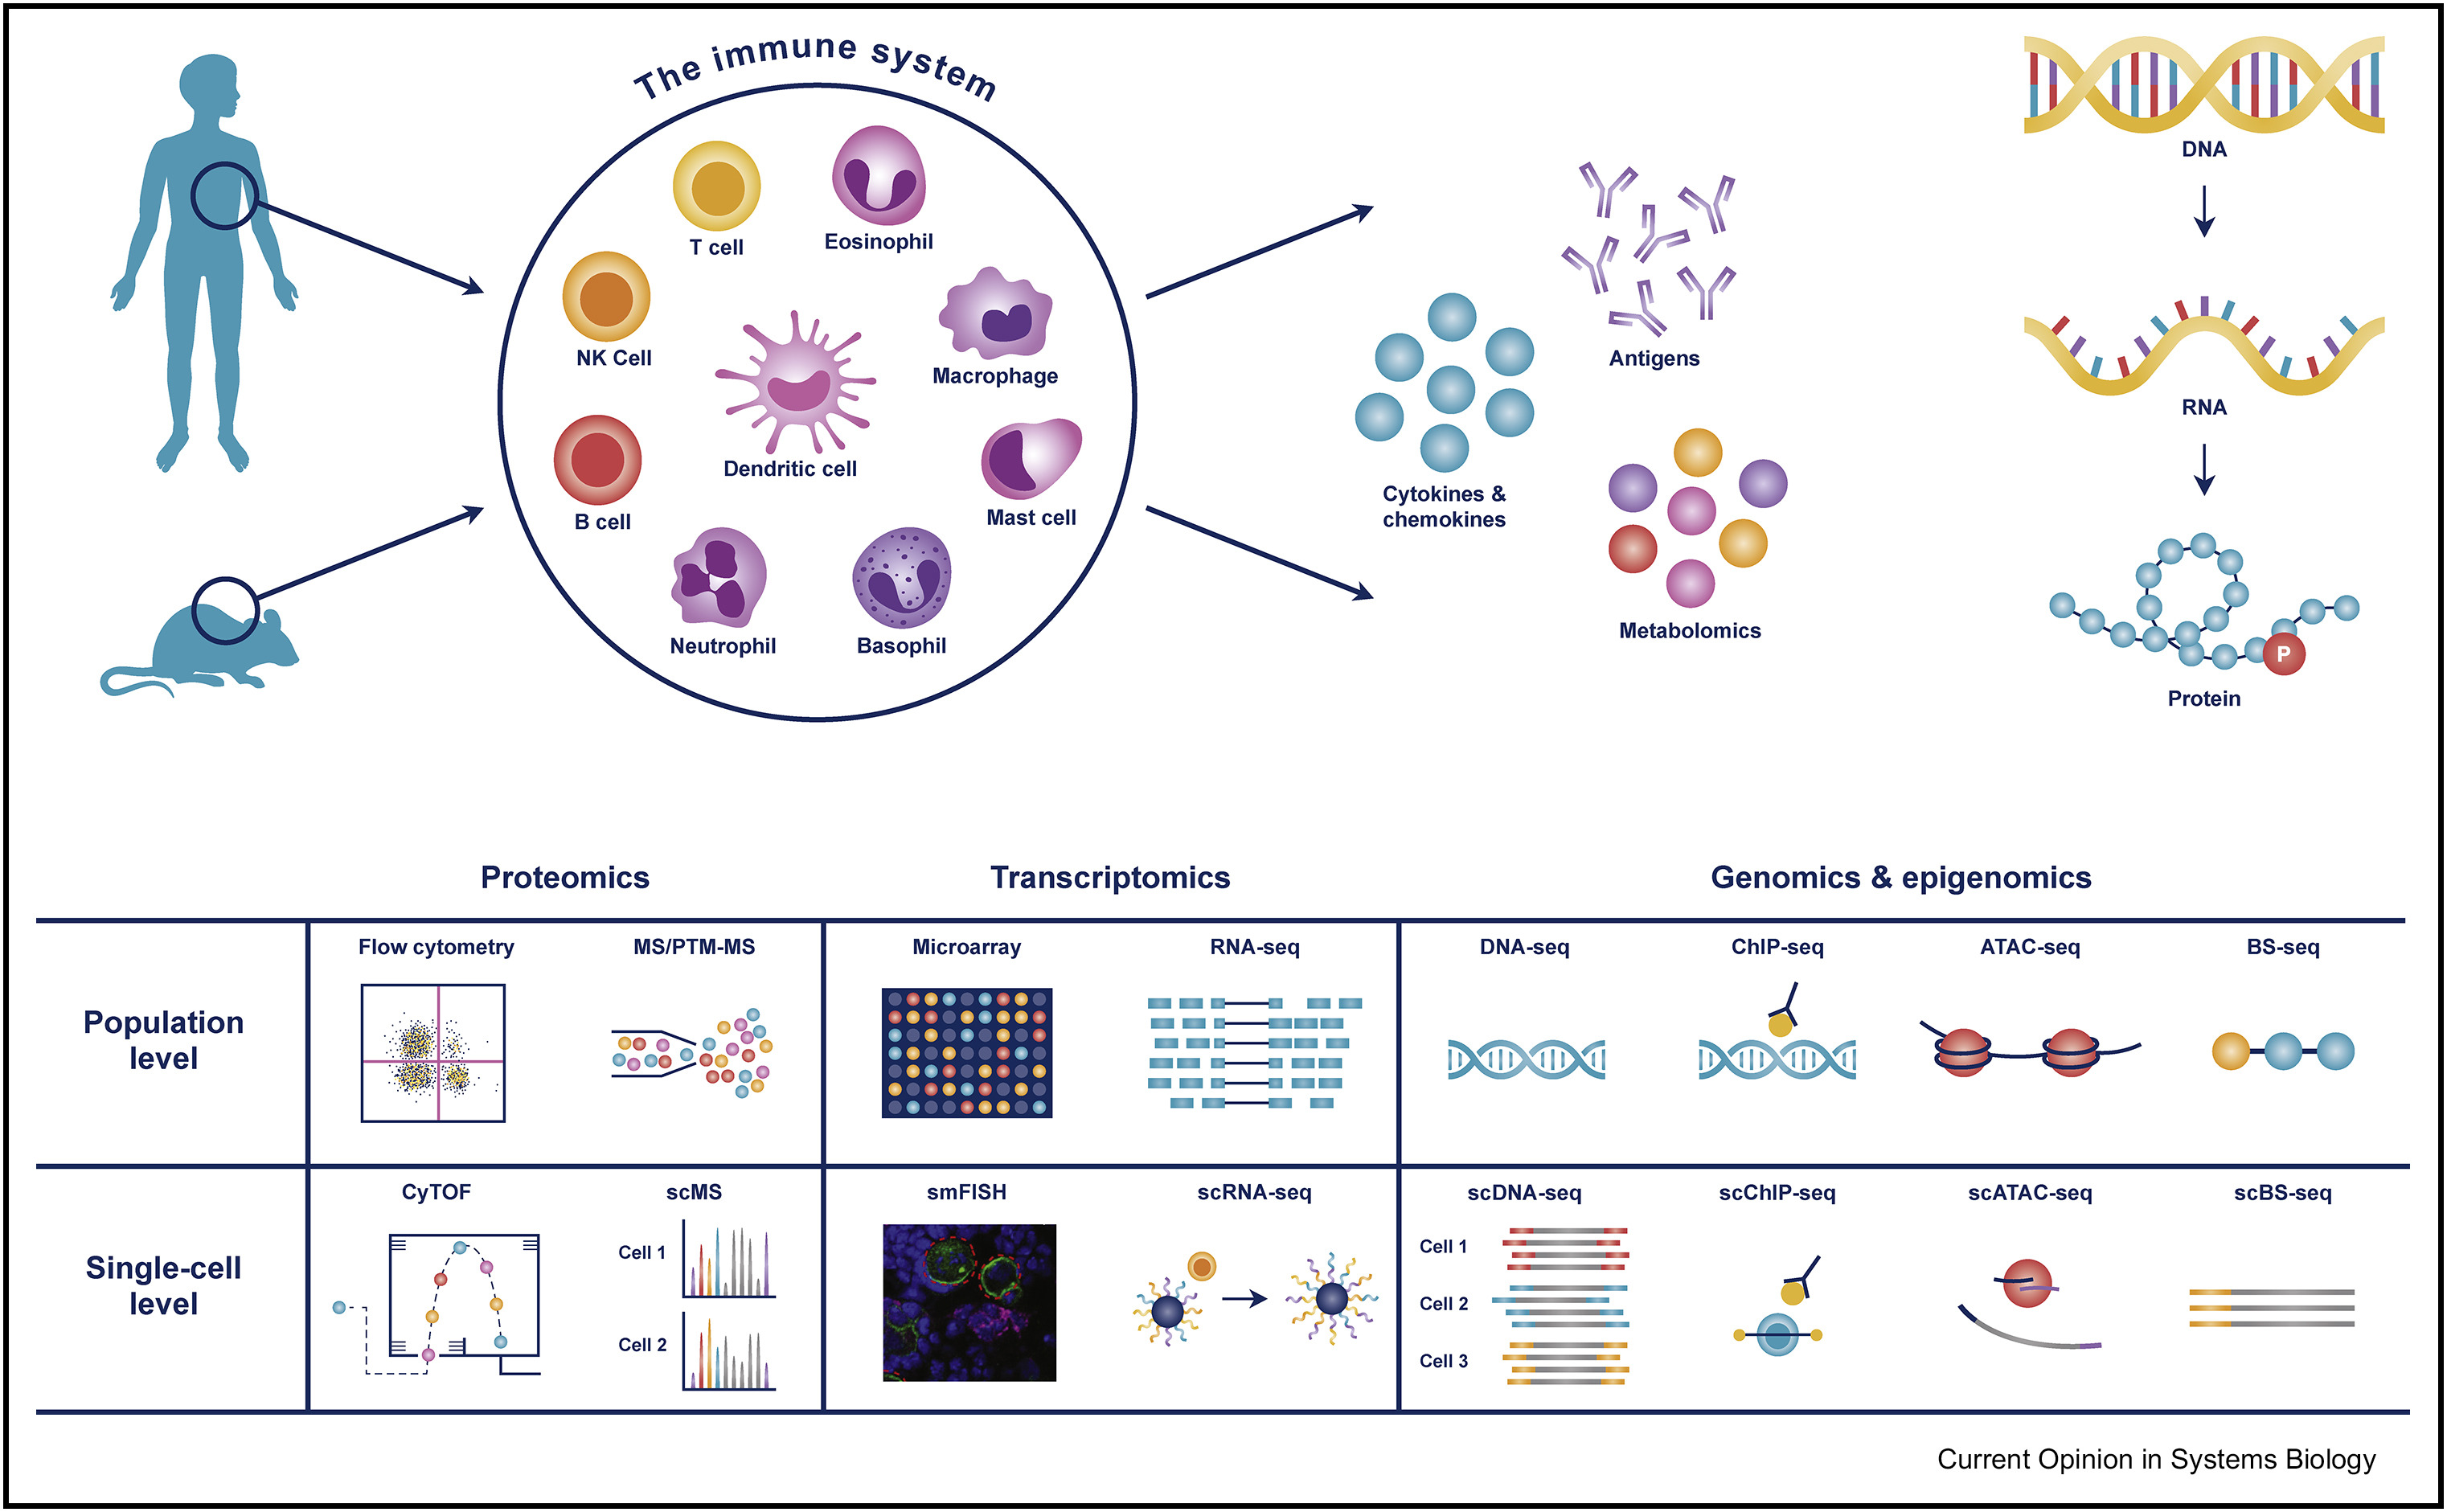
\includegraphics[width=1.0\textwidth,page=1]{mainmatter/figures/chapter_01/yu2019SystemsImmunologyIntegrating/1-s2.0-S2452310018301197-gr1_lrg.jpg}
    % TODO explain each technology in the figure legend
    \caption[
        \captionshort{High-throughput technologies for systems immunology.}
    ]{
        \textbf{High-throughput technologies for systems immunology.}
        Profiling can be done in humans and model organisms, at multiple levels of the immune system, and at bulk or single-cell resolutions.
        An additional dimension not shown here is profiling at multiple timepoints before and after perturbation.
        Figure reprinted from \textcite{yu2019SystemsImmunologyIntegrating}, \textcopyright~2019, with permission from Elsevier.
    }
    \label{fig:intro_sysImmunology}
\end{figure}

There are three major themes to systems immunology.
Initial studies of immune response to a particular perturbation are often descriptive,
aiming to find correlations between components of the immune response.
% or between immune components and higher-level phenotypic responses (e.g. cytokine and antibody levels).
Predictive studies then evaluate the ability to use measurements of relevant components to predict individual responses to the perturbation.
Feature sets that are molecular phenotypes (e.g. gene expression) with validated predictive accuracy are known as molecular signatures.
Causal inference is the third and most difficult goal.
Fortunately, the heritability of immune parameters (e.g. cell counts, surface marker expression, serum protein levels) is substantial (\SIrange{20}{40}{\percent} \autocite{liston2016ShapingVariationHuman,brodin2017HumanImmuneSystem,patin2018NaturalVariationParameters,liston2018OriginsDiversityHuman}),
with greater heritability for innate than adaptive immune parameters \autocite{patin2018NaturalVariationParameters}.
Much akin to \gls{GWAS} and \gls{QTL} studies, to identify causal links in the immune system,
one can leverage genetic variants as naturally-occurring perturbations \autocite{tsang2015UtilizingPopulationVariation,villani2018SystemsImmunologyLearning}.
Controlled variation can also be systematically generated by RNA interference or genome editing \autocite{yosef2016WritLargeGenomic}.
Obtaining causal understanding is essential for clinical translation,
to determine the interventions that can be made to promote effective response to pathogens and vaccines,
and impede pathways that lead to immune dysregulation in disease.
%
% TODO: add example high-profile study for each theme
% end with vaccine example and link to ch2 review as sysvac is major part of sysimm
% An established subfield is ...

% \subsection{Genetic effects on the healthy immune system}
%
% \1 Heritability of immune phenotypes is not only restricted to the expression phenotypes discussed above.
%     \2 Systems studies of interindividual variation in the healthy immune system shows many aspects of the immune system are heritable and complex.
%         \3 <Systems immunology: just getting started \url{https://www.nature.com/articles/ni.3768}>
%     \2 Immune parameters are influenced by age, sex, seasonality, and chronic infection \autocite{brodin2015VariationHumanImmune,liston2016ShapingVariationHuman,brodin2017HumanImmuneSystem,patin2018NaturalVariationParameters,liston2018OriginsDiversityHuman} \url{https://www.nature.com/articles/ncomms8000},
    % TODO: define aspects, parameters
    % TODO: add https://www.nature.com/articles/ni.3371 "The cellular composition of the human immune system is shaped by age and cohabitation"
%     but most individuals have a healthy baseline immune state that is individual-specific,
%     and relatively stable over time \autocite{liston2016ShapingVariationHuman,brodin2017HumanImmuneSystem,lakshmikanth2020HumanImmuneSystem}.
    % TODO: stable, yet varies by age? respecify scale of stability
    % TODO: add https://www.sciencedirect.com/science/article/abs/pii/S0952791520300698 "Understanding immune variation for improved translational medicine"
%     \2 Overall estimates of the heritability of many immune parameters, such as cell composition and serum protein levels, lies between 20-40\% \autocite{liston2016ShapingVariationHuman,brodin2017HumanImmuneSystem,patin2018NaturalVariationParameters,liston2018OriginsDiversityHuman}
%     \2 Genetic regulation is more important for the innate immune system than the adaptive immune system \autocite{patin2018NaturalVariationParameters}.
%
% \1 given genetic control of healthy system, perhaps not surprising that immune response to perturbation traits are also complex
%     \2 also, as discussed in the context section above, context-dependent genetic effects may not be apparent in the baseline healthy state, stimulation is required
%     \2 since a central goal of systems immunology is to establish causal relationships between the many components of the immune system
%         \3 Natural genetic variation can be leveraged as natural perturbations, representing small scale perturbations that are causally anchored \autocite{tsang2015UtilizingPopulationVariation,villani2018SystemsImmunologyLearning}
%     \2 In this context, immune in vivo reQTL studies can be considered as controllable perturbation studies of the activated immune system
%         \3 Studies of natural infection are complicated by e.g. determining exposure, ethics, dose
%     \2 Simultaneously provides insight in to the biology behind those specific responses
%     \2 Two immune perturbations considered in this thesis are vaccines and biologic drugs.

% \subsection{Immune response to anti-TNF biologics}
%
% TODO: merge this into intro ch4
% \1 <quick anti-tnf summary, specific ADA/IFX biology goes in ch4>
%     \2 biologics are drugs synthesised using a living organism, typically proteins
%     \2 cause immune response due to having immune targets, or immunogenecity because or their large and complex structure vs chem synth small molecule drugs
%     \2 one of the largest classes are anti-TNFs
%     \2 anti-TNFs (or TNF inhibitors), are drugs that suppress the activity of the TNF signalling pathway of the immune system
        % \3 TNF is an inflammatory cytokine ... inflammation is ...
%     \2 they are used to treat immune-mediated inflammatory diseases e.g. rheumatoid arthritis, Crohn's disease, psoriasis and ankylosing spondylitis.
    % Currently, five biologic agents targeting TNF are approved for the treatment of rheumatoid arthritis (RA), inflammatory bowel disease (IBD; for example, Crohn disease and ulcerative colitis), psoriasis, psoriatic arthritis, ankylosing spondylitis, juvenile idiopathic arthritis (JIA) and, most recently, hidradenitis suppurativa4,5 (TABLE 1).
%         \3 indicated for many IMIDs e.g. rheumatoid arthritis, Psoriasis, ankylosing spondylitis. \autocite{lichtenstein2013ComprehensiveReviewAntitumor,kalliolias2016TNFBiologyPathogenic,mulhearn2019UsingImmunophenotypePredict}
%     \2 an enormous amount of money is spent on them: anti-TNF biologics are some of the largest market share pharmaceuticals
%     \2 some proportion of patients fail. given the expenditures, it would be good to predict this
%
% TODO: figure on TNF pathway with drug targets
% TODO: table of biologics with costs
%
% TODO: merge this intro discussion ch4
% \1 <expression signatures of response to anti-TNFs>
%     \2 Systems immunology has also been applied to anti-TNFs
%     \2 have been detected e.g. for RA <"Validation study of existing gene expression signatures for anti-TNF treatment in patients with rheumatoid arthritis" \url{https://pubmed.ncbi.nlm.nih.gov/22457743/}>
    % e.g. https://www.ncbi.nlm.nih.gov/pmc/articles/PMC6614444/
%     \2 most detected in small cohorts, many require validation
%
% TODO: merge this intro discussion ch4
% \1 <genetics of anti-TNF response>
%     \2 pharmacogenomics is the study of the role of genetics in beneficial and adverse effects of drugs and theraputics \url{https://doi.org/10.1016/S0140-6736(19)31276-0}
%     \2 some implementation in clinic already e.g. screening for certain allele-drug combos \url{https://www.nature.com/articles/nature15817} \url{https://academic.oup.com/bmb/article/124/1/65/4430783}
%     \2 GWAS in the pharmacogenomics field \url{https://www.ncbi.nlm.nih.gov/pmc/articles/PMC3003940/} \url{https://www.futuremedicine.com/doi/full/10.2217/pgs-2018-0204}
    % Genome-wide association studies (GWAS) have proven to be a more successful approach for this objective. To date, eight GWAS on anti-TNF response in RA have been performed (22–29), identifying several loci associated at a genome-wide scale. From these, variation at MED15, GFRA1, PDE3A-SLCO1C1, and CD84 has been replicated in, at least, an independent cohort of patients (30).
%     \2 GWAS studies of anti-TNF response in RA \url{https://www.ncbi.nlm.nih.gov/pmc/articles/PMC6614444/}
        % \3 also add Discovery studies from \url{https://www.ebi.ac.uk/gwas/efotraits/EFO_0004653}
    % \2 TODO: \url{https://www.ebi.ac.uk/gwas/search?query=TNF},
    % also google anti tnf immune response gwas
        % e.g.
        % https://www.ncbi.nlm.nih.gov/pmc/articles/PMC6150911/
        % https://journals.plos.org/plosone/article?id=10.1371/journal.pone.0213073
%         \3 a few validation studies attempted e.g. \url{https://www.ncbi.nlm.nih.gov/pmc/articles/PMC5937760/}
%
% \1 a lot of studies also done for CD and IBD (described in ch4)

\section{Thesis outline}

This thesis examines longitudinal response to \textit{in vivo} immune perturbations by vaccines and drugs.
\Cref{ch:hird_DGE} is a descriptive \gls{DGE} study of transcriptomic and antibody responses to pandemic influenza vaccine (Pandemrix) in the \gls{HIRD} cohort of healthy adults.
\Cref{ch:hird_reQTL} integrates \gls{HIRD} genotype data to map the regulation of expression response to Pandemrix using an \textit{in vivo} \gls{reQTL} study design.
In \cref{ch:multiPANTS}, I mirror the design of the previous two chapters, 
exploring clinical response to biologic anti-\gls{TNF} therapy for \gls{CD} patients in the \gls{PANTS} cohort.
Finally, \cref{ch:discussion} presents an overview of shared themes and limitations,
and provides recommendations for future analyses and study designs for immune response phenotypes.
%
